\newpage
\section{Limiti funzioni in più variabili}
Restringiamoci nel caso di funzioni in 2 variabili; data una funzione $f: \mathbb{R}^2 \to \mathbb{R}$, una variabile $(x,y) \in \mathbb{R^2}$ e vogliamo dare un senso a $\lim\limits_{(x,y) \to (x_0, y_0)}f(x)$ con $(x_0, y_0) \in \mathbb{R^2}$. Ci aspettiamo 4 possibilità:
\begin{enumerate}
    \item Il limite esiste ed è finito (definizione \ref{def-1}).
    \item Il limite esiste ed è uguale a $+\infty$ (definizione \ref{def-2}).
    \item Il limite esiste ed è uguale a $-\infty$ (definizione \ref{def-3}).
    \item Il limite non esiste (quindi ne il punto 1 ne il 2 ne il 3 valgono).
\end{enumerate}

\begin{definition}\label{def-1}
Si dice che $\lim\limits_{(x,y) \to (x_0, y_0)} f(x,y) = +\infty$ con una $f: \mathbb{R}^2 \to \mathbb{R}$ e con $(x_0, y_0) \in \mathbb{R^2}$ se $\forall \: M \in \mathbb{R}$ (anche molto grande) $\exists \: \delta > 0$ tale che $f(x,y) \geq M \:\forall \: (x,y) \in B_{\delta}((x_0, y_0)) \setminus \{(x_0, y_0)\}$.
\end{definition}

\begin{definition}\label{def-2}
Si dice che $\lim\limits_{(x,y) \to (x_0, y_0)} f(x,y) = -\infty$ con una $f: \mathbb{R}^2 \to \mathbb{R}$ e con $(x_0, y_0) \in \mathbb{R^2}$ se $\forall \: M \in \mathbb{R}$ (anche molto negativo) $\exists \: \delta > 0$ tale che $f(x,y) \leq M \:\forall \: (x,y) \in B_{\delta}((x_0, y_0)) \setminus \{(x_0, y_0)\}$.
\end{definition}

\begin{figure}[h!]
\centering
\begin{subfigure}{.45\textwidth}
    \centering
    \includegraphics[width=4cm]{images/limiti-più-variabili-+inf.png}
    \caption{Definizione \ref{def-1}}
\end{subfigure}
\begin{subfigure}{.45\textwidth}
    \centering
    \includegraphics[width=4cm]{images/limiti-più-variabili--inf.png}
    \caption{Definizione \ref{def-2}}
\end{subfigure}
\end{figure}

\begin{definition}\label{def-3}
Si dice che $\lim\limits_{(x,y) \to (x_0, y_0)} f(x,y) = l \in \mathbb{R}$ con una $f: \mathbb{R}^2 \to \mathbb{R}$ e con $(x_0, y_0) \in \mathbb{R^2}$ se $\forall \: \epsilon > 0$ (anche molto piccolo) $\exists \: \delta > 0$ tale che $|f(x,y) - l| \leq \epsilon \:\forall \: (x,y) \in B_{\delta}((x_0, y_0)) \setminus \{(x_0, y_0)\}$.
\end{definition}

\begin{definition}[Funzione continua]
Una funzione $f: \mathbb{R}^n \to \mathbb{R}$ si dice \textbf{continua} in un punto $x_0 \in \mathbb{R}^n$ (che in questo caso indica un vettore), se $\lim\limits_{x\to x_0}f(x) = f(x_0)$, ($x \in \mathbb{R}^2$ è un vettore).
\end{definition}

\begin{definition}
Una funzione $f: \mathbb{R}^n \to \mathbb{R}$ è continua in tutto $\mathbb{R}^n$ se è continua $\forall \: x \in \mathbb{R}^2$.
\end{definition}
\hspace{-15pt}In generale la regola è che ogni funzione ottenuta a partire delle funzioni elementari usando operazioni algebriche e o usando composizioni è continua dove non presenta problemi di "esistenza" (per esempio il logaritmo $\leq 0$).

\begin{observation}
Gli strumenti standard del calcolo dei limiti che studiati nell'analisi fino ad ora, continuano ad essere validi per funzioni $f: \mathbb{R}^n \to \mathbb{R}$, unicità limite, la somma il prodotto ed il quoziente del limite, il teorema dei carabinieri, la permanenza del segno, teorema del confronto ecc.
\end{observation}

\hspace{-15pt}Per fare un confronto fra analisi in una variabile e quella in più variabili facciamo uno schema:
\begin{table}[h!]
    \centering
    \setlength{\tabcolsep}{7pt}
    \renewcommand{\arraystretch}{1.7}
    \begin{tabular}{|c|c|}
    \hline
    Analisi in una variabile & Analisi in più variabili \\\hline
    \makecell{    $f: \mathbb{R}\to \mathbb{R}$, $\lim\limits_{x\to x_0}f(x) = l \in \mathbb{R}$\\
    se $\forall \epsilon > 0 \:\exists\: \gamma > 0$ tale che $\forall \:x \::\: |x - x_0|< \gamma$,\\
    $x \neq 0$ vale che $|f(x) - l| \leq \epsilon$} & \makecell{$f: \mathbb{R}^n \to \mathbb{R}, x \in \mathbb{R}^n, x_0 \in \mathbb{R}^n, \lim\limits_{x\to x_0}f(x) = l$\\ se $\forall \: \epsilon > 0 \: \exists \: \gamma > 0$ tale che $\forall \: x \::\: ||x-x_0|| < \gamma,$\\
    $x \neq x_0$ vale $|f(x) - l| \leq \epsilon$}\\\hline
    \end{tabular}
\end{table}

Possiamo vedere che se confrontiamo queste due definizioni, formalmente, sono la stessa definizione, cambia che in una variabile abbiano un valore assoluto mentre in più variabili abbiamo una norma.

\begin{observation}
Anche se la struttura della definizione di limite rimane praticamente inalterata a meno di sostituire il valore assoluto con la norma, il calcolo dei limiti per funzioni di più variabili è più complicato. Questo perché in $\mathbb{R}, x$ tende ad un punto $x_0$ lungo una direzione data, mentre in $\mathbb{R}^n, x\in \mathbb{R}^n$ può tendere ad un punto $x_0 \in \mathbb{R}^n$ con n gradi di libertà.
\end{observation}

\subsection{Dimostrazione della non esistenza di un limite}
\begin{example}
Vediamo alcuni esempi nel caso di $f: \mathbb{R}^2 \to \mathbb{R}$.\\
Consideriamo ad esempio $\lim\limits_{(x,y) \to (0,0)}\frac{xy}{x^2 + y^2}$, quindi la nostra funzione è $f(x,y) = \frac{xy}{x^2 + y^2}$.\\
Esistono "diversi modi" di avvicinarsi all'origine (0,0). Però se $\exists\:\lim\limits_{(x,y) \to (0,0)}\frac{xy}{x^2 + y^2} = l \in \mathbb{R}$ allora il limite (per sua unicità) non deve dipendere dalla direzione di avvicinamento a (0,0).\\
Prova a dire che $\nexists \:\lim\limits_{(x,y) \to (0,0)}\frac{xy}{x^2 + y^2}$ (non esiste), a seconda della direzione di avvicinamento il limite cambia, ma questo contraddice l'unicità del limite. Vediamo come possiamo avvicinarsi:
\begin{itemize}
    \item Avvicinarsi lungo l'asse x: $y=0$, quindi sto guardando la funzione $f(x,0)$ quindi la funzione $f$ solo sui punti dell'asse x. Quindi se mi restringo all'asse x ho $\lim\limits_{x\to 0}f(x,0) = 0$.
    \item Lungo l'asse y: $x=0$, quindi ho $f(0,y) = 0$ che è una funzione dove guardo solo i punti dell'asse y allora $\lim\limits_{y \to 0}f(0,y) = 0$.
    \item Lungo bisettrice $y=x$, quindi sto guardando $f(x,x)$ cioè sto guardando la funzione solo sui punti tale che $y=x$, quindi $f(x,x) = \frac{x^2}{2x^2} = \frac{1}{2}$ e quindi è costante e quindi $\lim\limits_{x\to 0}f(x,x) = \frac{1}{2}$.\\
    Questa cosa si può fare anche con la bisettrice $x = y$ che da l'ho stesso risultato ma anche con $x = -y$ e $y = -x$.
\end{itemize}
\end{example}
\begin{wrapfigure}[9]{r}{6cm}
\vspace{-20pt}
    \centering
    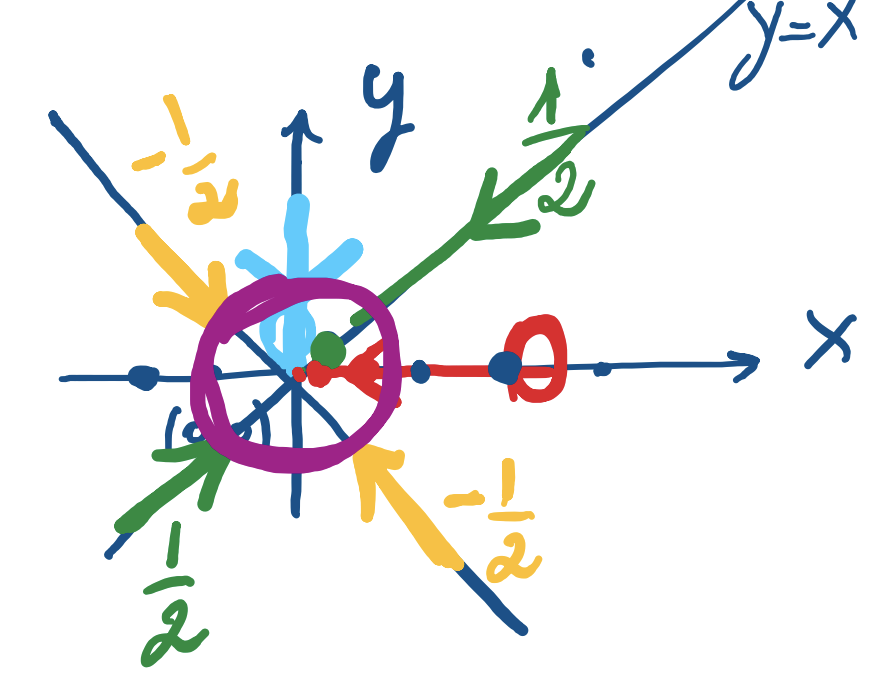
\includegraphics[width=5cm]{images/ess-lim-2var-asseX.png}
\end{wrapfigure}
Ho quindi trovato almeno 2 direzioni di avvicinamento (asse x e la bisettrice $y=x$) che mi danno 2 limiti diversi (0 e $\frac{1}{2}$) ma visto che il limite se esiste sarebbe unico il limite non esiste.\\
In ogni palla di centro (0,0) trovo punti in cui $f$ vale 0 e punti in cui $f$ vale $\frac{1}{2}$ allora il limite non esiste.
\hspace{-15pt}In generale possiamo dimostrare che un limite non esiste andando a trovare due direzioni di avvicinamento in cui il limite è diverso. In $\mathbb{R}^n$ capita molto spesso che i limiti non esistano, molto più spesso del caso di una singola variabile.

\begin{example}
Prendiamo ora $\lim\limits_{(x,y)\to (0,0)}f(x,y)$ con $f(x,y) = \frac{x}{||(x,y)||}$,
\end{example}
\begin{wrapfigure}[4]{r}{5cm}
\vspace{-35pt}
    \centering
    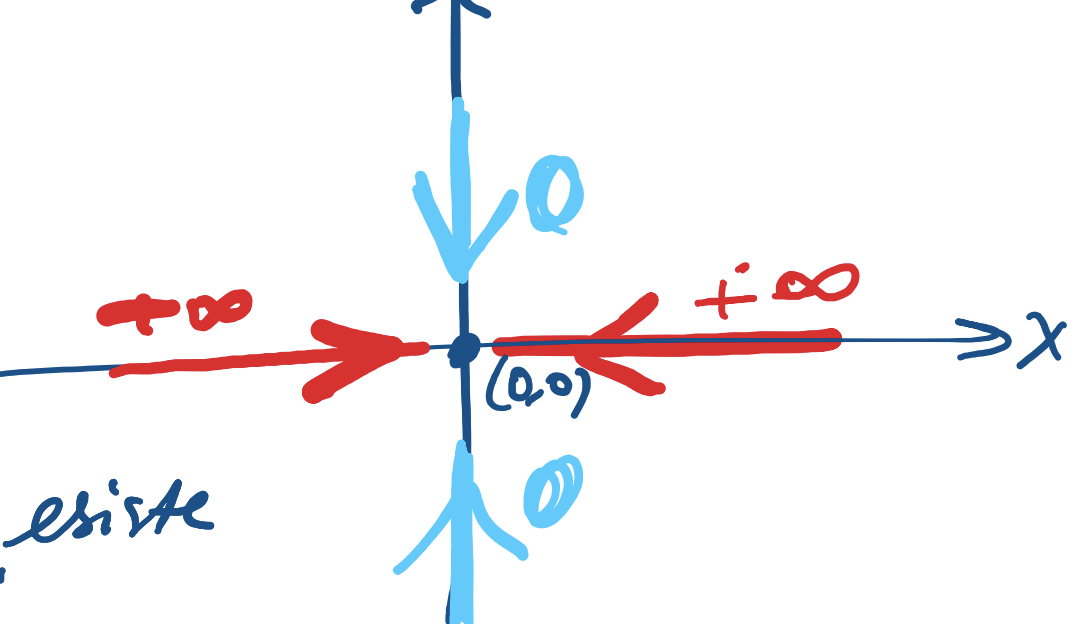
\includegraphics[width=4cm]{images/ess-lim-2var-2.png}
\end{wrapfigure}
che possiamo scrivere anche come $f(x,y) = \frac{x}{x^2 + y^2}$, dobbiamo anche in questo caso bisogna dimostrare che il limite non esiste. Per dimostrare che non esiste cerco due direzioni di avvicinamento all'origine (0,0) con due limiti diversi.
\begin{itemize}
    \item Lungo l'asse x: $y = 0$ quindi vuol dire che sto guardando la funzione $f(x,0) = \frac{x}{x^2} = \frac{1}{x}$ e quindi il $\lim\limits_{x\to 0}f(x,0) = +\infty$.
    \item Lungo l'asse y: $x=0$ vuol dire che ho $f(0,y) = \frac{0}{y^2} = 0$ e quindi $\lim\limits_{y \to 0}f(0,y) = 0$.
\end{itemize}
Bastano dunque queste due direzioni con il limite diverso per concludere che il limite non esiste.


\begin{note}
Attenzione: se provo diverse direzioni e mi viene sempre lo stesso limite questo non basta per concludere che il limite esiste perché potrebbe esserci una direzione che io non ho ancora esplorato che mi da limite diverso.
\end{note}

\begin{example}
Vediamo un esempio della casistica descritta nella nota. $f(x,y) = \frac{x^2 \cdot y}{x^4 + y^2}$ e voglio guardare $\lim\limits_{(x,y) \to (0,0)}f(x,y)$. Proviamo allora a guardare delle direzioni:
\begin{enumerate}
    \item Lungo l'asse x: $y = 0$ stiamo guardando la funzione $f(x,0) = 0$ quindi $\lim\limits_{x\to 0}f(x,0) = 0$.
    \item Lungo l'asse y: $x = 0$ quindi consideriamo al funzione $f(0,y) = 0$ quindi $\lim\limits_{y \to 0}f(0,y) = 0$.
    \item Lungo bisettrice $y= x$: in questo caso $f(x,x) = \frac{x^2 - x}{x^4 + x^2} = \frac{x^2}{x^4 + x^2} = \frac{x}{x^2 + 1}$ e quindi $\lim\limits_{x\to 0}f(x,x) = 0$.
    \item Lungo le rette del tipo $y = mx$: stiamo guardando allora $f(x,mx) = \frac{x^2 \cdot mx}{x^4 + m^2x^2} = \frac{mx}{x^2 + m^2}$, in questo caso qualunque sia $m \in \mathbb{R}^2$ posso concludere che $\lim\limits_{x\to 0}\frac{mx}{x^2 + m^2} = 0$.
\end{enumerate}
\end{example}
\begin{wrapfigure}[8]{l}{5cm}
    \vspace{-10pt}
    \centering
    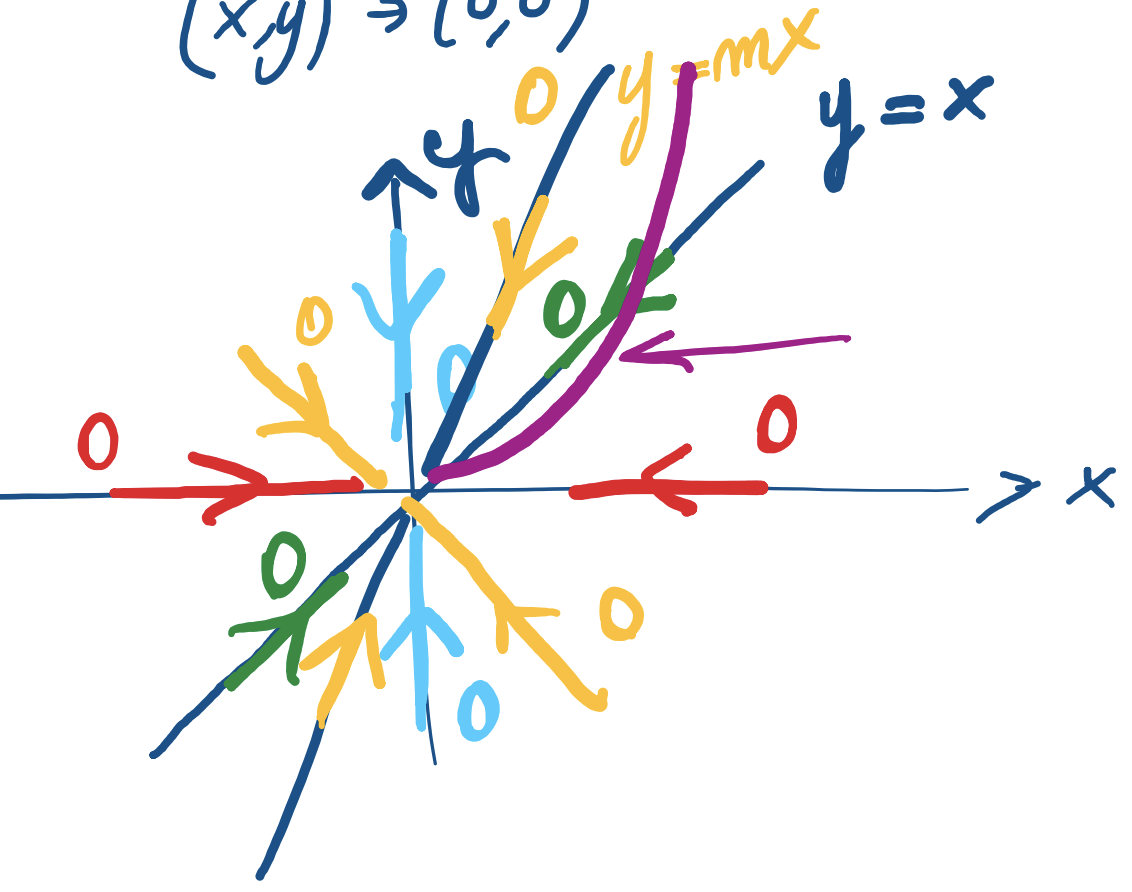
\includegraphics[width=4.3cm]{images/ess-lim-2var-3.png}
\end{wrapfigure}
Nonostante abbiamo visto che lungo tutte le direzioni di avvicinamento provate il limite è 0 questo non basta a concludere che il limite esiste perché ne ho provate solo alcune. Proviamo infatti adesso ad avvicinarsi all'origine lungo la parabola $y = x^2$. Se restringiamo $f$ a questa parabola stiamo guardando $f(x, x^2) = \frac{x^2 \cdot x^2}{x^4 + x^4} = \frac{x^4}{2x^4}= \frac{1}{2}$ ma quindi $\lim\limits_{x\to 0}f(x, x^2) = \frac{1}{2} \neq 0$ e quindi abbiamo trovato un caso in cui il limite è diverso e quindi posso concludere per l'unicità del limite che non esiste.


\subsection{Calcolo limiti con teoremi}
Proviamo a studiare $\lim\limits_{(x,y)\to (0,0)}\frac{x^2 y^6}{x^2 + y^2}$ con $f: \mathbb{R}^2 \to \mathbb{R}$ come prima cosa proviamo a fare il limite classico sostituendo ma che fa si che venga $\frac{0}{0}$ che è una forma indeterminata.\\
Osservo che $\frac{x^2 y^6}{x^2 + y^2}$ è una funzione sempre positiva inoltre posso scrivere $\frac{x^2 y^6}{x^2 + y^2} = y^6 \cdot \frac{x^2}{x^2 + y^2}$ possiamo vedere che il termine $\frac{x^2}{x^2 + y^2} \leq 1$ perché denominatore $\geq$ numeratore, quindi abbiamo che $y^6 \cdot \frac{x^2}{x^2 + y^2} \leq y^6$ quindi risulta che $0 \leq f(x,y) \leq y^6$ possiamo usare il teorema dei carabinieri dove $0 \to 0$ e $y^6 \to 0$ quindi concludiamo che $\lim\limits_{(x,y)\to (0,0)}f(x,y) = 0$.

\subsection{Calcolo limiti con cambio di variabile}
Calcoliamo $\lim\limits_{(x,y) \to (0,0)}\frac{\sin(x^2 + y^2)}{(x^2 + y^2)} = \frac{0}{0}$ che è una forma indeterminata. Possiamo in questo caso usare il cambio di variabile, pongo quindi $t = x^2 + y^2$, quindi ho che quando $(x,y)\to (0,0)$ ho che $t \to 0$ quindi riscrivo il limite come $\lim\limits_{t\to 0}\frac{\sin{t}}{t} = 1 \Longrightarrow \lim\limits_{(x,y)\to (0,0)} \frac{\sin(x^2+y^2)}{x^2+y^2} = 1$.

\subsection{Regola valore assoluto}
Prendiamo ora il limite $\lim\limits_{(x,y)\to (0,0)}\frac{x^2y}{x^2 + y^2}$, in questo ci verrebbe da usare come visto prima il teorema dei carabinieri però non possiamo perché abbiamo a moltiplicare un $y$ che quando cambia segno la funzione cambia segno, dobbiamo quindi usare la regola del valore assoluto.
\begin{proposition}[Regola del valore assoluto]
Data una funzione $f: \mathbb{R}^2 \to \mathbb{R}$ se $|f(x,y)| \to 0$ allora anche $f(x,y) \to 0$
\end{proposition}
\begin{demostration}
Questo perché $-|f(x,y)| \leq f(x,y) \geq |f(x,y)|$ quindi è come dire che $-|a| \leq a \leq |a|$ e quindi se il minorane ed il maggiorante tendono a 0 per il teorema dei carabinieri anche $f(x,y)$ tende a 0.
\end{demostration}
\vspace{-5pt}
\hspace{-15pt}Applichiamolo quindi al nostro caso con $f(x,y) = \frac{x^2 \cdot y}{x^2 + y^2}$ e quindi $|f(x,y)| = \bigg| \frac{x^2 \cdot y}{x^2 + y^2} \bigg| = |y| \cdot \frac{x^2}{x^2 + y^2}$ perché $\frac{x^2}{x^2 + y^2} \geq 0$ e quindi viene influenzata solo da $y$. quindi abbiamo che $0 \leq |f(x,y)| = |y| \cdot \frac{x^2}{x^2+y^2} \leq |y|$ quindi $|y| \to 0$ e per il teorema dei carabinieri $|f(x,y)| \to 0$ e per la regola del valore assoluto $f(x,y) \to 0$.

\subsection{Metodo delle coordinate polari}
Questo è un metodo che facilità il calcolo dei limiti in $\mathbb{R}^2$. \\
Abbiamo $(x,y) \in \mathbb{R}^2$ che sono dette coordinate cartesiane ma esistono anche quelle dette coordinate polari definite come $(\rho,\Theta)$ con $\rho \in \mathbb{R}, \Theta \in \mathbb{R}$. Le coordinatore polari e le cartesiane sono legate nel seguente modo: $x = \rho \cos{\Theta}, y = \rho \sin{\Theta}$\\
Le coordinate polari hanno il seguente vantaggio: la condizione $(x,y)\to 0$ in termini di coordinate polari diventa $\rho \to 0$. Il metodo prevede di esprimete la funzioni in termini di coordinate polari, quindi ne nostro caso $f(x,y) = \frac{x^2y}{x^2 + y^2} = \frac{\rho^2\cos{\Theta}^2 \cdot \rho\sin{\Theta}}{\rho^2 \cos{\Theta}^2 + \rho^2\sin{\Theta}^2} = \frac{\rho^3 \cos{\Theta}^2 \cdot \sin{\Theta}}{\rho^2} = \rho \cos{\Theta}^2 \cdot \sin{\Theta}$ ho quindi espresso la funzione con $\rho$ e $\Theta$.\\
Vediamo ora che $\lim\limits_{(x,y)\to (0,0)}\frac{x^2y}{x^2 + y^2} = \lim\limits_{\rho \to 0}f(\rho, \Theta) = \rho \cos{\Theta}^2 \cdot \sin{\Theta}$ quindi devo fare un limite in una variabile e posso quindi procedere facendo come fatto nell'analisi ad una variabile. Vediamo quindi che $-\rho \leq \rho \cos{\Theta}^2 \cdot \sin{\Theta} \leq \rho$ visto che $\cos{\Theta}^2 \leq 1$ e $-1 \leq \sin{\Theta} \leq 1$, usano il teorema dei carabinieri abbiamo che $-\rho \to 0$, $\rho \to 0$ e quindi $\rho \cos{\Theta}^2 \cdot \sin{\Theta} \to 0$.

\begin{example}
Facciamo un altro esempio di questo metodo prendendo $f(x,y) = \frac{xy}{x^2 + y^2}$ e usandolo per dimostrare che per $(x,y)\to (0,0)$ il limite non esiste. Ricordiamo che $x = \rho\cos{\Theta}$ e $y = \rho\sin{\Theta}$ e quindi $f(\rho, \Theta) = \frac{\rho\cos{\Theta} \cdot \rho\sin{\Theta}}{\rho^2\cos{\Theta}^2 + \sin{\Theta}^2} = \frac{\rho^2\cos{\Theta} \cdot \sin{\Theta}}{\rho^2} = \cos{\Theta}\sin{\Theta}$. Quindi $\lim\limits_{(x,y)\to (0,0)}f(x,y) = \lim\limits_{\rho\to 0^+}f(\rho, \Theta) = \lim\limits_{\rho\to 0^+}\cos{\Theta}\sin{\Theta} = \cos{\Theta}\sin{\Theta}$ che quindi dipende da $\Theta$ e quindi non è un numero e quindi non esiste un limite finito in $\mathbb{R}$.
\end{example}

\begin{example}
Sia data una funzione $f: \mathbb{R}^2 \to \mathbb{R}$ definita come $f(x,y) = \begin{cases}\frac{x^4 + y^3}{x^2 + y^2} & (x,y) \neq (0,0)\\ a & (x,y) = (0,0)\end{cases}$, questo esercizio ci chiede di trovare $a \in \mathbb{R}$ tale che $f$ sia continua in $(0,0)$. Questo vuol dire che la soluzione corrisponderà a cercare $a \in \mathbb{R}$ (vedere innanzitutto se esiste) tale che $\lim\limits_{(x,y)\to (0,0)}f(x,y) = a$.\\
Quindi calcoliamo il $\lim\limits_{(x,y)\to (0,0)}\frac{x^4 + y^3}{x^2 + y^2} = \frac{0}{0}$ forma indeterminata. Questo è un caso in cui è possibile utilizzare le coordinate polari, ricordiamo che $x = \rho \cos{\Theta}, y = \rho \sin{\Theta}$, e che $\lim\limits_{(x,y)\to (0,0)} = \lim\limits_{\rho\to 0}$. \\
Scriviamo quindi la funzione con le coordinate polari: $f(\rho,\Theta) = \frac{\rho^4\cos{\Theta}^4 + \rho^3\sin{\Theta}^3}{\rho^2\cos{\Theta}^2 + \rho^2\sin{\Theta}^2} = \frac{\rho^4\cos{\Theta}^4 + \rho^3\sin{\Theta}^3}{\rho^2} = \frac{\rho^2(\rho^2\cos{\Theta}^4 + \rho\sin{\Theta}^3)}{\rho^2} = \rho^2\cos{\Theta}^4 + \rho\sin{\Theta}^3$.\\
Ora voglio calcolare $\lim\limits_{\rho \to 0}f(\rho, \Theta) = \rho^2\cos{\Theta}^4 + \rho\sin{\Theta}^3$, posso vedere che $\cos{\Theta}^4 \leq 1 \:\forall \:\Theta$ e $\sin{\Theta}^3 \leq 1 \:\forall \:\Theta$ sono due funzioni limitate per due funzioni $\rho^2, \rho \to 0$. Posso quindi affermare che $\exists\: \lim\limits_{(x,y)\to (0,0)}f(x,y) = 0$, $f$ è continua in $(0,0) \Longleftrightarrow a = 0$ abbiamo quindi concluso.
\end{example}

\subsection{Limiti che vanno a $\infty$}
Finora abbiamo visto limiti $\lim\limits_{(x,y)\to(x_0,y_0)}f(x,y)$ con $(x_0,y_0)\in \mathbb{R}^2$ fissato, quindi con un valore finito ed nel caso in cui la funzione sia definita in tutto $\mathbb{R}^2$.
\begin{observation}
Nel caso fosse definita in un sottoinsieme $f: \Omega \to \mathbb{R}$ con $\Omega \subset \mathbb{R}^2$ stessa definizione ma $(x_0,y_0)$ deve essere un punto di accumulazione per l'insieme $\Omega$.
\end{observation}
\hspace{-15pt}Ora però ci chiediamo come si estende la nozione di limite quando $\lim\limits_{(x,y)\to \infty}f(x,y) = l$. Innanzitutto dobbiamo chiederci cosa voglia dire $(x,y)\to \infty$; ricordiamo che un intorno di raggio r di $\infty$ è il complementare di $B_r((0,0))$, quindi $(x,y)\to \infty$ se la d($(x,y),0$)$\to +\infty$, che posso esprimerlo come $x^2 + y^2 \to +\infty$ oppure $\rho \to +\infty$.

\begin{definition}[Limite finito che tende a $\infty$]
Si dice che $\lim\limits_{(x,y)\to \infty}f(x,y) = l \in \mathbb{R}$ se $\forall \: \epsilon > 0$ esiste un intorno di $\infty$ tale che se $(x,y)$ appartiene all'intorno allora $|f(x) - l|\leq \epsilon$. In maniera più formale si può dire che esiste se $\forall \: \epsilon > 0 \:\exists\: \delta > 0$ tale che se $(x,y) \notin B_{\gamma}(0,0)$ allora $|f(x,y) - l| \leq 0$.
\end{definition}

\begin{definition}[Limite infinito che tende a $\infty$]
Si dice che $\lim\limits_{(x,y)\to \infty}f(x,y) = +\infty \in \mathbb{R}$ se $\forall \: M > 0$ esiste se $\exists\: \delta > 0$ tale che se $\forall \: (x,y) \notin B_{\gamma}(0,0)$ vale $f(x,y) \geq M$. Lo stesso vale per $-\infty$ ma considerando $f(x,y) \leq M$.
\end{definition}
\hspace{-15pt}Anche nel caso di $\lim\limits_{(x,y)\to \infty}f(x,y)$ valgono le seguenti cose:
\begin{itemize}
    \item Se esistono due direzioni con limite diverso allora non esiste il limite.
    \item Le coordinate polari possono semplificare il calcolo.
\end{itemize}

\begin{example}
Consideriamo $\lim\limits_{(x,y)\to +\infty}\frac{y^6}{1 + x^2 + y^2}$. Fare questo limite equivale a fare $\lim\limits_{x^2 + y^2\to +\infty} \Longleftrightarrow \lim\limits_{\rho\to +\infty} \Longleftrightarrow \lim\limits_{d((x,y),0)\to +\infty}$. Sappiamo che possiamo tendere all'infinito in diversi modi, quindi vado ora a scegliere diversi direzioni di avvicinamento:
\begin{itemize}
    \item Mi avvicino dall'asse x, quindi $y=0$ e quindi $(x,y)\to \infty$ con $y=0$ corrisponde a $x^2 \to +\infty$ il che equivale a $d((x,0),(0,0))\to +\infty$. Se quindi $y=0$ la nostra funzione $f(x,y) = f(x,0) = \frac{0}{1+x^2} \to 0$.
    \item Se scegliamo come direzione di avvicinamento ad $\infty$ l'asse y quindi $x=0$ allora $\lim\limits_{(x,y)\to +\infty}f(x,y) = \lim\limits_{y^2 \to \infty}\frac{y^6}{1 + y^2}$, ma questo limite è uguale a $\lim\limits_{y^2 \to \infty}\frac{y^6}{1 + y^2} = +\infty$.
\end{itemize}
Quindi lungo l'asse x viene 0 mentre lungo l'asse y torna $\infty$, quindi ho trovato 2 direzioni con due diversi valori del limite e quindi risulta che il limite non esiste.
\end{example}

\begin{example}
Prendiamo $\lim\limits_{(x,y)\to \infty}xye^{-(x^2 + y^2)}$. Come sempre vale che il limite vale per $\lim\limits_{x^2 + y^2\to +\infty} \Longleftrightarrow \lim\limits_{\rho\to +\infty} \Longleftrightarrow \lim\limits_{d((x,y),0)\to +\infty}$. In questo caso per calcolare il limite ci viene comodo passare alle coordinate polari, quindi $f(\rho, \Theta) = \rho\cos{\Theta}\cdot \rho\sin{\Theta} \cdot e^{-\rho^2} = \sin{\Theta}\cos{\Theta} \cdot \frac{\rho^2}{e^{\rho^2}}$.\\
Noi, essendo passati a coordinate polari, vogliamo calcolare $\lim\limits_{\rho \to +\infty}\sin{\Theta}\cos{\Theta} \cdot \frac{\rho^2}{e^{\rho^2}}$, notiamo che il fattore $\frac{\rho^2}{e^{\rho^2}}$ dipende solo da $\rho$ mentre $\sin{\Theta}\cos{\Theta}$ dipende solo da $\Theta$ ma è limitato, sappiamo che $\frac{\rho^2}{e^{\rho^2}}\to 0$ che moltiplica con una moltiplicata e quindi $f(\rho,\Theta) \to 0$, quindi $\lim\limits_{\rho \to +\infty}\sin{\Theta}\cos{\Theta} \cdot \frac{\rho^2}{e^{\rho^2}} \to 0$ e quindi $\lim\limits_{(x,y)\to \infty}xye^{-(x^2 + y^2)} \to 0$.
\end{example}
